%\section{Empricial Experiments}

\section{Evaluating Enhanced Techniques}
\label{sec:evaluation}

This section evaluates the enhanced downstream
testing techniques on real-world subject programs
that contain test dependence.

\subsection{Subject Programs}

use the same subject programs

\subsection{Methodology}

%\subsubsection{Understanding Dependence Root Causes}

%results
\begin{figure}[t]
%\hspace{0.5cm}
\begin{minipage}[b]{\linewidth}
\centering
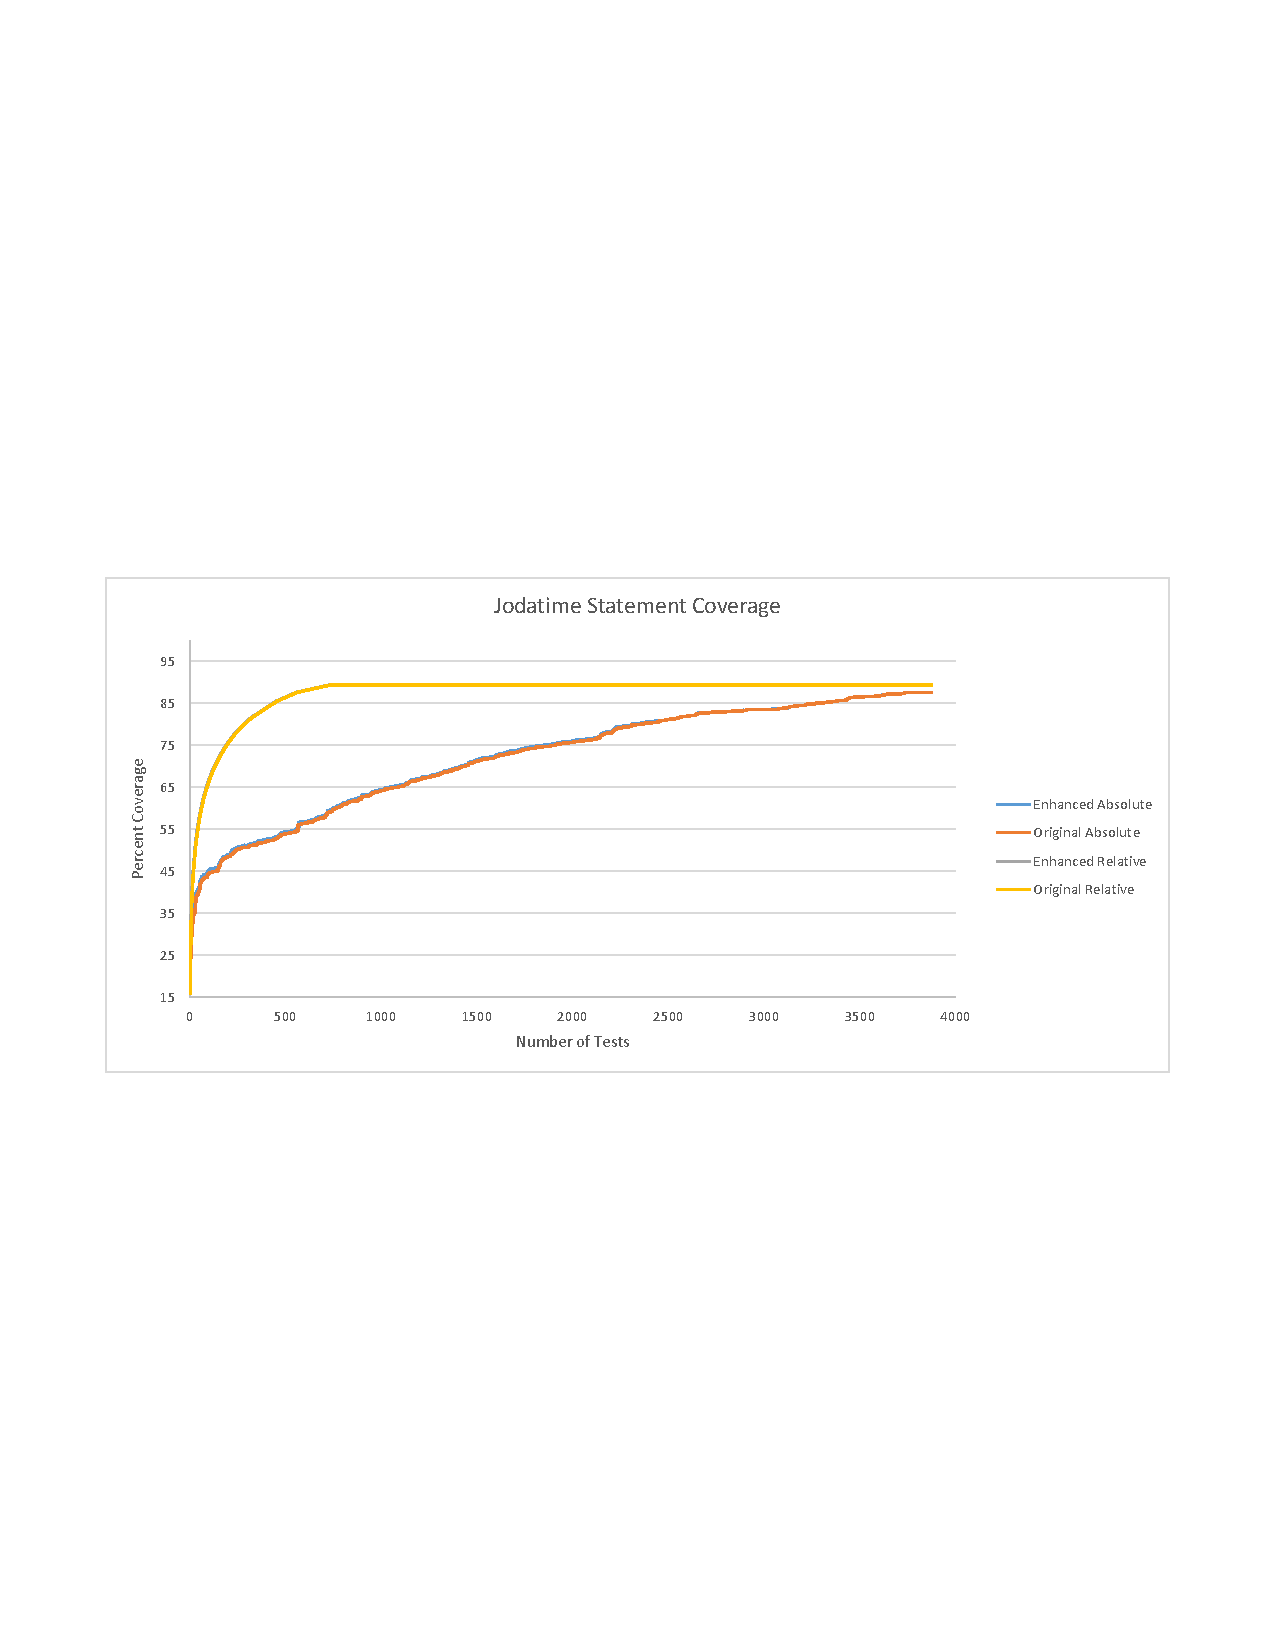
\includegraphics[scale=0.46]{jodatime-coverage-figure}
Jodatime
%\caption{replace} \label{fig:p2}
\end{minipage}
\begin{minipage}[b]{\linewidth}
\centering
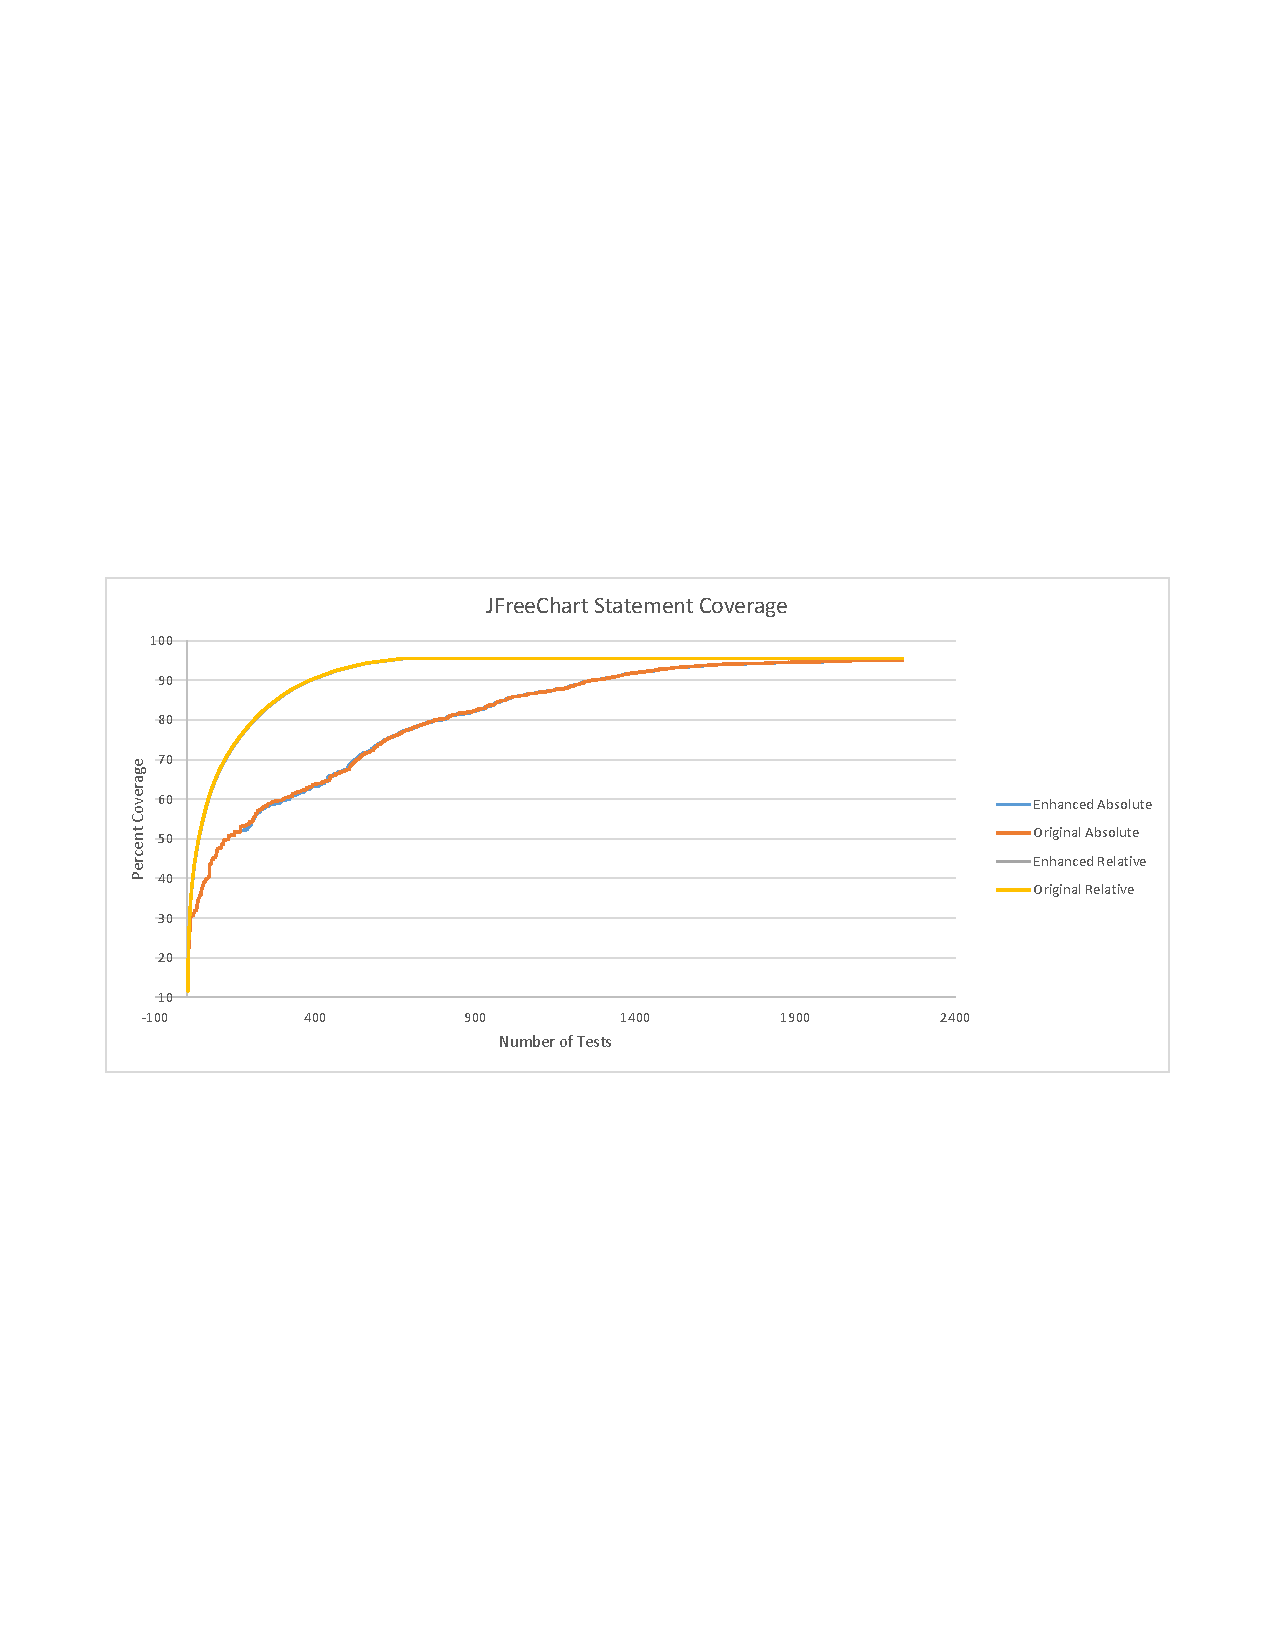
\includegraphics[scale=0.46]{jfreechart-coverage-figure}
JFreechart
%\caption{schedule} \label{fig:p3}
\end{minipage}
\begin{minipage}[b]{\linewidth}
\centering
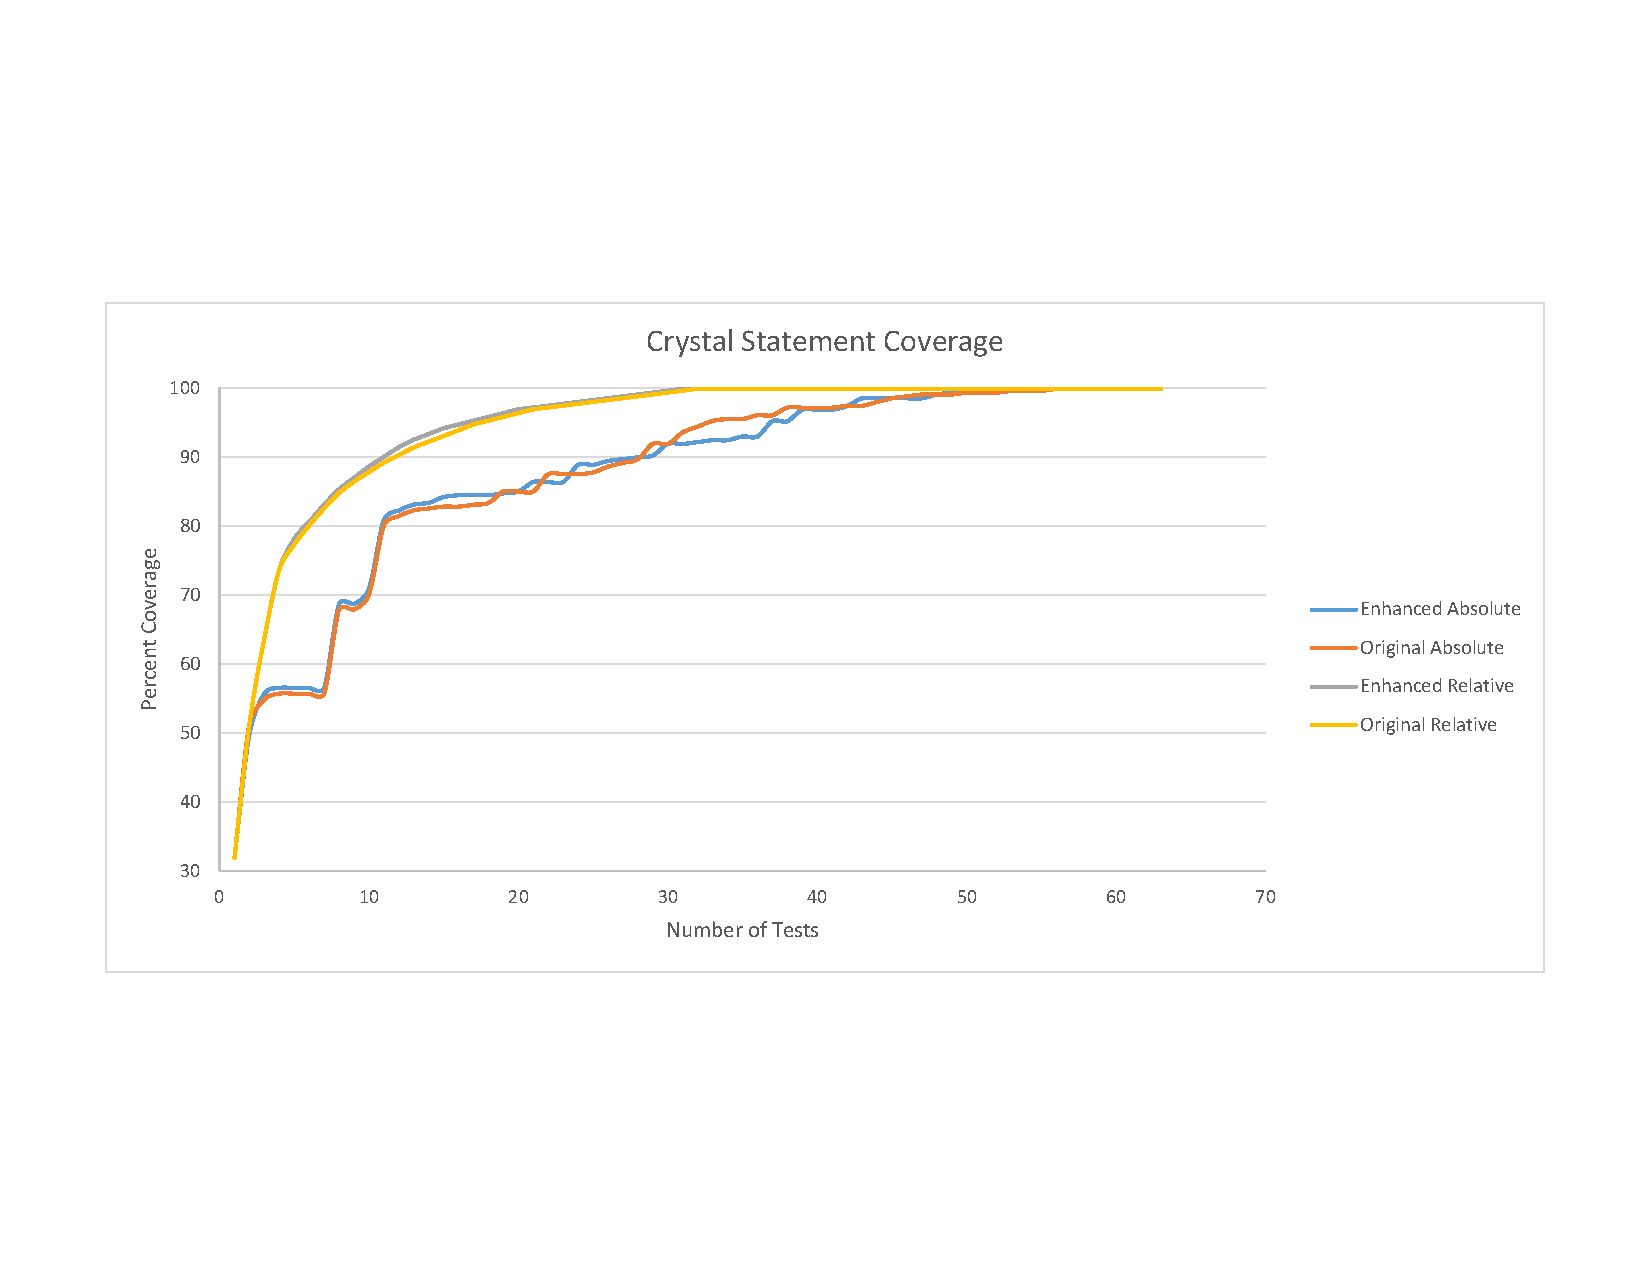
\includegraphics[scale=0.35]{crystal-coverage-figure}
{Crystal}
%\caption{tcas} \label{fig:p1}
\end{minipage}
\vspace{-6mm}
\caption{
    \label{fig:results}
Statement coverage results by each test prioritization technique on
our evaluation subject programs. \todo{explain why some is missing} }
\end{figure}




\subsection{Dependance-Aware Test Prioritization}

\subsection{Dependance-Aware Test Selection}

\begin{table}
\centering
\setlength{\tabcolsep}{1.25\tabcolsep}
\begin{tabular}{|l|c|c|}
%\toprule
\hline
\textbf{Subject Program} & S1 (statement-level) & S2 (method-level)  \\
\hline
\multicolumn{3}{|l|}{}  \\
\multicolumn{3}{|l|}{\textbf{Human-written Test Suites}}  \\
\hline
\jt& 332 $\rightarrow$ 335 & 3233 $\rightarrow$ 3233 \\
XML Security& 70 $\rightarrow$ 83 & 71 $\rightarrow$ 84  \\
%\bottomrule
\hline
\textbf{Total} & 402 $\rightarrow$ 418 & 3304 $\rightarrow$ 3317 \\
\hline
%\textbf{Total}& &  & &  \\ 
%\hline
\end{tabular}
\caption{Results of evaluating the \selnum test selection techniques
in Table~\ref{tab:enhancetestsel} on four human-written unit test suites.
Each cell shows the number of selected tests.
}
\label{tab:testselresult}
\end{table}


\subsection{Dependance-Aware Test Parallelization}

\begin{table*}
\centering
\setlength{\tabcolsep}{1.25\tabcolsep}
\begin{tabular}{|l| l|l|l|l| l|l|l|l| l|l|l|l|}
%\toprule
\hline
\textbf{Subject Program} & \multicolumn{4}{|l|}{P1 (Original Order Parallelization)} &  \multicolumn{4}{|l|}{P2 (Random Parallelization)} & \multicolumn{4}{|l|}{P3 (Time-Minimized Parallelization)}\\
\cline{2-13}
& k=2 & k=4 & k=8 & k=16 & k=2 &k=4& k=8& k=16 & k=2 &k=4& k=8& k=16\\
\hline
\multicolumn{13}{|l|}{}  \\
\multicolumn{13}{|l|}{\textbf{Human-written Test Suites}}  \\
\hline
\jt& 3.47 & 1.97 & 1.84 & 1.80 & 2.83 & 2.61 & 1.92 & 1.80 & 2.20 & 2.11 & 1.38  & 1.79\\
XML Security& 1.45 & 1.89 & 2.48 & 5.72 & 1.56  & 2.35 & 4.02  & 4.25 & 2.56 & 2.82  & 4.38 & 6.00 \\
Crystal& 1.72  & 1.84  & 1.24  & 1.48  & 1.72 & 2.16& 1.72 & 1.04 & 2.12 & 1.34 & 1.33& 1.26\\
JFreechart&  1.33 & 1.26 & 1.15  & 1.27  & 1.44 & 1.28 & 1.30 & 1.22 & 1.46 & 1.31 & 1.31 & 1.40\\
%\bottomrule
\hline
\textbf{Average} & 1.99  & 1.74 & 1.67  & 2.57 & 1.89 & 2.10& 2.24 & 2.08 & 2.09 & 1.89 & 2.10 & 2.61\\
\hline
%\textbf{Total}& &  & &  \\ 
%\hline
\end{tabular}
\caption{Results of evaluating the enhanced test parallelization techniques
on the subject programs.
\todo{show the slow, explain why synoptic does not work}
}
\label{tab:testparresult}
\end{table*}


\subsection{Discussion}

\subsubsection{Threats to Validity}

There are several threats to the validity
of our experiments. First, \dtexplain 
only considers test dependencies arised
from improper field access. It may not
produce useful results for other types of
test dependencies~\cite{}. Second,
\todo{evaluating on the test coverage, no
bug finding abilities yet.}

\subsubsection{Experimental Conclusions}

We have two chief findings. \textbf{(1)} \dtexplain
generates concise report to explain why
test dependence arises, and such report
helps developers to understand the root cause
of test dependence. \textbf{(2)} All
enhanced downstream testing techniques
output consistent results on test suites
containing dependent tests.
